\documentclass[10pt]{article} % For LaTeX2e
\usepackage{tmlr-template/tmlr}
% If accepted, instead use the following line for the camera-ready submission:
%\usepackage[accepted]{tmlr}
% To de-anonymize and remove mentions to TMLR (for example for posting to preprint servers), instead use the following:
%\usepackage[preprint]{tmlr}

\input{tmlr-template/math_commands}

\usepackage{hyperref}
\usepackage{url}
\usepackage{graphicx}
\usepackage{amsmath}
\usepackage{amssymb}


\usepackage{bm}

\def\vTheta{{\bm{\Theta}}}
\def\vPhi{{\bm{\Phi}}}
\newcommand{\dambiguity}{\mathcal{A}_{\mathrm{D}}}
\newcommand{\pambiguity}{\mathcal{A}_{\mathrm{P}}}
\newcommand{\pperformance}{\mathcal{E}_{\mathrm{P}}}
\newcommand{\dperformance}{\mathcal{E}_{\mathrm{D}}}
\newcommand{\sg}{\operatorname{sg}}

\title{Sparse Ensembles: Do Routing Mechanisms Benefit from Ensemble Effects?}

% Anonymous submission
\author{Anonymous Author(s)}

\newcommand{\fix}{\marginpar{FIX}}
\newcommand{\new}{\marginpar{NEW}}

\def\month{MM}
\def\year{YYYY}
\def\openreview{\url{https://openreview.net/forum?id=XXXX}}

\begin{document}

\maketitle

\begin{abstract}
Ensemble effects among predictive models have been studied extensively and are a well-established source of improved generalization. In sparse ensembles, however, prediction is only one part of the problem: inputs must also be routed to the appropriate models. Whether this routing mechanism itself benefits from ensemble effects remains largely unexplored. We provide a systematic study of ensembling the routing mechanism, examining when increasing the number of routers improves performance, how their outputs should be combined, and whether explicitly encouraging diversity among routers is beneficial. Across classification and regression tasks, we characterize how these choices interact with the size and capacity of the underlying models and the routing ensemble.

\end{abstract}

\section{Introduction}

Ensemble methods are a well-established class of machine learning techniques that improve generalization by aggregating the predictions of multiple models. Their effectiveness is typically attributed to two complementary factors: the performance of the individual predictors and the diversity among them. Improving individual predictors reduces bias, while diversity promotes  error de-correlation, allowing aggregation to cancel out model-specific mistakes.

Classical ensemble methods induce diversity implicitly via bagging, such as random forests, where predictors are trained on different subsets of the data, whereas boosting methods, such as LightGBM, construct predictors sequentially to focus on errors made by earlier models. In deep learning, diversity can be encouraged explicitly through mechanisms such as negative-correlation learning \citep{chen_ncl_weight} or expert orthogonalization \citep{liu2024diversifying}. However, \citet{fort2019deep} showed that, in many cases, initializing experts with different random weights is sufficient to induce substantial diversity.

Sparse ensembles, in which only a subset of predictors is active for a given input, have gained prominence because of their computational advantages in large-scale language modeling. In the most prominent setting, each expert, or subset of experts, is responsible for a particular region of the input domain, allowing the ensemble to approximate the capacity of a larger model while retaining the computational cost of a smaller one. Existing variants balance computation and ensemble effects in different ways: selecting the top-$k$ predictors for each input \citep{shazeer2017outrageously}, maximizing cost reduction by routing each input to a single predictor \citep{fedus2022switch}, or allocating a dynamic number of predictors per input \citep{wang2025remoe}. Routing-based methods decompose prediction into two coupled subproblems: a \textit{delegation problem}, handled by a \textit{router} or \textit{delegator}, and a \textit{prediction problem}, handled by the \textit{experts} or \textit{predictors}.

While ensembles typically focus on improving the predictive capacity of the experts, the delegation mechanism itself may also benefit from ensembling. This motivates studying whether increasing the number of delegators improves the allocation of unseen samples to predictors and, consequently, the overall performance of the ensemble. Despite recent methods that combine multiple routers \citep{zhang2025mixture, ran2025router}, the effect of scaling the number of delegators remains underexplored. In particular, to our knowledge, there is no systematic analysis of this setting through the lens of ensemble theory.

\paragraph{Contributions} In this work we provide a systematic study of scaling the number of delegators in image classification tasks, focusing on CIFAR10 \citep{krizhevsky2009learning} and SVHN \citep{netzer2011reading}, and tabular regression tasks, Bike sharing dataset \citep{bike_sharing_275} and Energy production dataset \citep{energydataset}. Specifically this work systematically tests scaling of number of delegators, number of predictors, delegator widths, and predictor widths. Furthermore, two aggregation methods are tested, probabilities product and probabilities sum. We find:

\begin{itemize}
    \item \textbf{(C1) When scaling number of delegators helps}: Under which scenarios
    \item \textbf{(C2) What aggregation method is better for the delegators}: Is sum better?
    \item \textbf{(C3) Ambiguity gradient control}: We examine how separately controlling predictor and delegator ambiguity gradients affects ensemble performance.
    \item \textbf{(C4) Predictor and delegator decompositions}: We formulate a performance--ambiguity decomposition for delegators through the predictions their weights induce, and use a restricted oracle to separate residual predictor loss from recoverable delegation loss.
   
\end{itemize}

\section{Background} \label{sec:background}

We consider a supervised learning setting with a training dataset $\sD = \{(\vx_n, \vy_n)\}_{n=1}^{N}$ of $N$ i.i.d.\ samples, where $\vx \in \sR^{d_x}$ denotes the input and $\vy \in \sR^{d_y}$ the corresponding real-valued output for regression, or $\vy \in \{0,1\}^{d_y}$ a one-hot target for classification. We write $\Delta_M = \{\va \in \sR^M : a_m \geq 0,\ \sum_{m=1}^M a_m = 1\}$ for the probability simplex.

We define an ensemble of $M$ predictors $f_m = f_{\vtheta_m}$, with parameters $\vTheta = (\vtheta_1,\ldots,\vtheta_M)$, and an ensemble of $L$ delegators $g_l = g_{\vphi_l}$, with parameters $\vPhi = (\vphi_1,\ldots,\vphi_L)$. A predictor produces an output vector $\hat{\vy}_m(\vx) = f_m(\vx)$, which is a probability vector for classification. A delegator produces a weight proposal $\va_l(\vx) = g_l(\vx) \in \Delta_M$. Thus, predictors estimate the target, while delegators determine how predictors are combined.

For any weights $\va \in \Delta_M$, define the predictor aggregate as prescribed in \citet{wood2023unified}:
\begin{equation}\label{eq:predictor-aggregate}
    F(\vx;\va) =
    \begin{cases}
        \displaystyle\sum_{m=1}^M a_m\hat{\vy}_m(\vx), & \text{regression},\\[2mm]
        \displaystyle\frac{\bigodot_{m=1}^M\hat{\vy}_m(\vx)^{a_m}}
        {\sum_{c=1}^{d_y}\prod_{m=1}^M \hat y_{m,c}(\vx)^{a_m}}, & \text{classification}.
    \end{cases}
\end{equation}
Here $\bigodot$ denotes componentwise multiplication and $\vv^{\odot a}$ denotes componentwise exponentiation. The delegator proposals are combined into $\bar{\va}(\vx) \in \Delta_M$ using either an arithmetic or normalized geometric mean (Section~\ref{sec:exp-agg}). For an input $\vx$, the final prediction is $\hat{\vy} = F(\vx;\bar{\va}(\vx))$, and the prediction induced by delegator $l$ alone is $\hat{\vy}^{(l)} = F(\vx;\va_l(\vx))$. With no delegators ($L=0$), we use uniform weights $\bar a_m = 1/M$.

\subsection{Predictor performance and ambiguity}

For a fixed sample $(\vx,\vy)$, write $\hat{\vy}_m=f_m(\vx)$ for each predictor's output. Let $\mathrm{SE}(\hat{\vy},\vy)=d_y^{-1}\|\hat{\vy}-\vy\|_2^2$ and $\mathrm{CE}(\hat{\vy},\vy)=-\sum_{c=1}^{d_y}y_c\log\hat y_c$ denote squared error and cross-entropy. For any weights $\va\in\Delta_M$, the classical squared-error decomposition \citep{NIPS1994_b8c37e33} is
\begin{equation}\label{eq:mse-train}
    \mathrm{SE}(F(\vx;\va),\vy)
    = \underbrace{\sum_{m=1}^M a_m\mathrm{SE}(\hat{\vy}_m,\vy)}
        _{\text{weighted predictor loss }\pperformance(\va)}
      -\underbrace{\sum_{m=1}^M a_m\mathrm{SE}(F(\vx;\va),\hat{\vy}_m)}
        _{\text{weighted predictor ambiguity }\pambiguity(\va)}.
\end{equation}
For cross-entropy with geometric aggregation, the corresponding decomposition is \citep{wood2023unified}
\begin{equation}\label{eq:ce-train}
    \mathrm{CE}(F(\vx;\va),\vy)
    = \underbrace{\sum_{m=1}^M a_m\mathrm{CE}(\hat{\vy}_m,\vy)}
        _{\text{weighted predictor loss }\pperformance(\va)}
      -\underbrace{\sum_{m=1}^M a_m\mathrm{KL}(F(\vx;\va)\,\|\,\hat{\vy}_m)}
        _{\text{weighted predictor ambiguity }\pambiguity(\va)}.
\end{equation}
In both cases, $\pperformance$ measures individual predictor accuracy, while $\pambiguity$ measures disagreement with the aggregate output. Lower individual loss and greater ambiguity at fixed individual loss improve ensemble performance. We use $\ell$ for the task loss (SE or CE) and $d$ for its ambiguity measure (SE or KL), so both identities read $\ell(F(\vx;\va),\vy)=\pperformance(\va)-\pambiguity(\va)$.

Explicit maximization of ambiguity has been shown to be potentially harmful, since it can increase the bias and variance of the individual models, leading to higher generalization error \citep{pmlr-v151-ortega22a, wood2023unified}. In contrast, prior work indicates that using different random initializations is often sufficient to induce test-time diversity among ensemble members \citep{fort2019deep, pmlr-v151-ortega22a}. This motivates controlling ambiguity gradients separately from the loss decomposition itself (Section~\ref{sec:exp-gradient}).

\section{Delegator decompositions}\label{sec:delegator-decompositions}

\subsection{Delegator performance and ambiguity}\label{sec:delegator-ambiguity}

There is no target weight vector for a delegator. Instead, we assess each proposal through the predictor ensemble it induces. The loss $\ell(\hat{\vy}^{(l)},\vy)$ measures whether delegator $l$ proposes weights that yield an accurate prediction. Its ambiguity $d(\hat{\vy},\hat{\vy}^{(l)})$ measures disagreement with the final prediction, rather than disagreement between weight vectors themselves.

For arithmetic aggregation $\bar{\va}=L^{-1}\sum_{l=1}^L\va_l$, the final prediction is also the appropriate equal-weight aggregate of the induced predictions: their arithmetic mean for regression and their normalized geometric mean for classification. Applying the classical ambiguity decomposition (Equations~\ref{eq:mse-train}--\ref{eq:ce-train}) to these predictions gives
\begin{equation}\label{eq:delegator-ambiguity}
    \ell(\hat{\vy},\vy)
    = \underbrace{\frac{1}{L}\sum_{l=1}^L\ell(\hat{\vy}^{(l)},\vy)}
        _{\text{individual delegator loss }\dperformance}
      -\underbrace{\frac{1}{L}\sum_{l=1}^L d(\hat{\vy},\hat{\vy}^{(l)})}
        _{\text{delegator ambiguity }\dambiguity}.
\end{equation}
The derivation for both tasks is given in Appendix~\ref{ap:delegator-decomposition}.
Thus, each delegator should propose weights yielding a good predictor ensemble, while diversity is measured in the outputs these proposals induce. A larger $\dambiguity$ is beneficial at fixed $\dperformance$. Each delegator's loss also has the predictor decomposition
\begin{equation}\label{eq:delegator-terms}
    \ell(\hat{\vy}^{(l)},\vy)
    = \pperformance(\va_l)-\pambiguity(\va_l).
\end{equation}
Equation~\ref{eq:delegator-ambiguity} does not generally hold for geometric aggregation of delegation weights. The two terms remain defined, but their difference need not equal the final loss. Both terms require $L\geq 1$.

\subsection{Delegator error}

We also separate the final loss into a predictor loss under reference weights and a delegation regret. This is distinct from the performance--ambiguity decompositions above. For fixed predictor outputs and a sample $(\vx,\vy)$, define the unrestricted oracle weights by
\begin{equation}
    \va^\star(\vx,\vy) \in \argmin_{\va\in\Delta_M}
        \ell(F(\vx;\va),\vy).
\end{equation}
The loss decomposes exactly as
\begin{equation}\label{eq:delegator-decomposition}
    \ell(\hat{\vy},\vy)
    = \underbrace{\ell(F(\vx;\va^\star),\vy)}_{\text{predictor loss under optimal weights}}
    + \underbrace{\big[\ell(\hat{\vy},\vy)-\ell(F(\vx;\va^\star),\vy)\big]}_{\text{delegator regret}}.
\end{equation}
The first term is the minimum loss attainable by any admissible delegation weights for the given predictor outputs; the second is nonnegative. For regression, the first term is the squared distance to the convex hull of $\{\hat{\vy}_m\}_{m=1}^M$, divided by $d_y$, and is zero exactly when the target lies in that hull. This convex-hull interpretation does not apply to geometrically aggregated classification probabilities.

The unrestricted, label-dependent oracle can be overly optimistic: with sufficiently many predictors, arbitrary sample-specific weights may interpolate regression targets. We therefore use a restricted delegator oracle with the same architecture as the learned delegators. With predictors fixed, this oracle seeks weights that reduce the ensemble loss. Its aggregate weights are denoted by $\va^\dagger(\vx)$. They provide a reference for attributing the remaining loss between predictors and delegators, but need not be optimal. The fitting and data-splitting procedure is described in Appendix~\ref{ap:restricted-oracle}.  

Replacing $\va^\star$ by $\va^\dagger$ gives
\begin{equation}\label{eq:restricted-delegator-decomposition}
    \ell(\hat{\vy},\vy)
    = \underbrace{\ell(F(\vx;\va^\dagger),\vy)}_{\text{predictor loss under restricted-oracle weights}}
    + \underbrace{\big[\ell(\hat{\vy},\vy)-\ell(F(\vx;\va^\dagger),\vy)\big]}_{\text{restricted delegator regret}}.
\end{equation}
The second term measures the difference relative to the restricted oracle and may be negative, since the oracle is not sample-wise optimal. The first term is the predictor loss remaining under that reference. Together, they distinguish potential gains from better delegation from the loss that remains after delegation is improved.

\section{Experiments}

Our claims are validated empirically over selection of four datasets: CIFAR10 \citep{krizhevsky2009learning}, SVHN \citep{netzer2011reading}, Bike sharing dataset \citep{bike_sharing_275}, and Energy production dataset \citep{energydataset}. For each dataset, the inputs $\vx$ and targets $\vy$ were normalized where applicable, and categorical integer-valued features were one-hot encoded. For each random seed, the data were independently partitioned into training and validation sets using an $85\%$--$15\%$ split. Each training run is repeated across 5 different seeds.

For the tabular regression tasks, Bike and Energy, we use fully connected MLPs with two hidden layers, and optimize them using the mean squared error loss, $\ell_{\mathrm{MSE}}$. The hidden-layer widths decrease progressively toward the output: the two-layer architecture uses widths $(2b, b)$, where $b$ is a model-specific base width. This parameterization preserves a consistent architectural shape while allowing the capacities of the predictor and delegator networks to be varied independently through their respective base widths. Regression tasks are learned for $2000$ epochs.

For the image-classification tasks, CIFAR-10 and SVHN, we use three-layer MLPs with hidden widths being $(3b, 2b, b)$, where $b$ is a model-specific base width. Classification tasks are optimized using the cross-entropy loss, $\ell_{\mathrm{CE}}$. Remaining training hyper-parameters are specified in Table \ref{tab:training-hyperparameters}. Image tasks are learned for $100$ epochs.

Following the load-balancing motivation of \citet{shazeer2017outrageously} and \citet{fedus2022switch}, we penalize nonuniform predictor usage through normalized Gini impurity. For a minibatch $\sB\subseteq\sD$, the final training objective is
\begin{equation}\label{eq:training-objective}
\begin{aligned}
    \mathcal{L}_{\sB}
    &= \frac{1}{|\sB|}\sum_{(\vx,\vy)\in\sB}\ell_{\mathrm{train}}(\vx,\vy)
       +\lambda\frac{\sum_{m=1}^M u_m^2-1/M}{1-1/M},\\
    \vu &= \frac{1}{|\sB|}\sum_{(\vx,\vy)\in\sB}\bar{\va}(\vx),
\end{aligned}
\end{equation}
where $M>1$, $\lambda=0.2$, and $\ell_{\mathrm{train}}$ has the value of the ensemble loss but the selected training gradients defined in Section~\ref{sec:exp-gradient}. This penalty encourages balanced predictor use across the minibatch.

The overall ensemble performance is evaluated on $\sD_{\mathrm{val}}$ using the unregularized loss $\ell(\hat{\vy},\vy)$. We further assess the individual performance and diversity of predictors through $\pperformance$ and $\pambiguity$, and of delegators through $\dperformance$ and $\dambiguity$. Finally, Equation~\ref{eq:restricted-delegator-decomposition} separates the remaining error into potential gains from improved delegation or improved prediction.

\subsection{Scaling the number of delegators} \label{sec:exp-scaling}

We next investigate whether delegation itself benefits from an ensemble effect, and under which model-capacity regimes such benefits emerge (Contribution \textbf{(C1)}). In particular, we study whether increasing the number of delegators is most useful when the predictor ensemble is small, the predictors have limited capacity, or the individual delegators are themselves relatively small.

To isolate the effect of the number of delegators, we vary $L \in \{0,1,2,4,8,16,32\}$ while exhaustively evaluating all combinations of the number of predictors $M \in \{2,4,8,16,32\}$, predictor base width $b_M \in \{4,8,16\}$, and delegator base width $b_L \in \{4,8,16\}$ across all four tasks. The case $L=0$ corresponds to fixed uniform delegation weights $\bar{\va}$, whereas $L=1$ recovers a setting closely related to a standard mixture-of-experts model. Each experimental condition is evaluated over five independent random seeds, yielding $6300$ training runs. We use the \texttt{Delegators} predictor-ambiguity setting (Section~\ref{sec:exp-gradient}) with delegator ambiguity disabled (Section~\ref{sec:exp-delegator-gradient}).

\subsection{Delegator's aggregation method} \label{sec:exp-agg}

Previous work \citep{pmlr-v151-ortega22a, wood2023unified} characterizes optimal aggregation rules for predictors under a fixed set of weights $\va$. In our setting, however, predictor and delegator parameters are optimized jointly. Consequently, the aggregation rule affects not only the final combination of delegator outputs, but also the optimization dynamics through which predictors and delegators co-adapt. Results derived for fixed-weight aggregation therefore do not directly determine the appropriate aggregation rule for delegators in our model. We therefore evaluate this choice empirically, corresponding to Contribution \textbf{(C2)}.

We compare two aggregation rules over the $L$ delegators: the arithmetic mean, $\bar{\va}(\vx) = L^{-1}\sum_{l=1}^{L}\va_l(\vx)$, and the normalized geometric mean, $\bar{\va}(\vx) = Z^{-1}\bigodot_{l=1}^{L}\va_l(\vx)^{L^{-1}}$, where $Z$ normalizes the weights to sum to one. The predictor aggregation in Equation~\ref{eq:predictor-aggregate} remains unchanged. We use the \texttt{None} predictor-ambiguity setting (Section~\ref{sec:exp-gradient}) with delegator ambiguity enabled (Section~\ref{sec:exp-delegator-gradient}).

To isolate the effect of the aggregation rule, we construct 100 experimental configurations by sampling the remaining experimental variables from the sets reported in Table~\ref{tab:experiment-parameters}. For each configuration and each of the four tasks, we evaluate a matched pair of experiments differing only in the delegator aggregation rule: arithmetic mean or geometric mean. This yields 800 experimental conditions. Each condition is evaluated over five independent random seeds, for a total of 4,000 training runs.

\subsection{Predictor Ambiguity gradient flow} \label{sec:exp-gradient}

As discussed in Section~\ref{sec:background}, explicitly maximizing predictor ambiguity can harm individual predictor performance. The standard training procedures suggest only to use the weighted performance $\pperformance$, however, the delegators still should identify decorrelated predictors using the predictor ambiguity $\pambiguity$. We therefore propose to include the ambiguity term $\pambiguity$ in the loss equation but to stop its gradient from influencing the predictor parameters $\vTheta$. We empirically compare three ways to train the predictor ensemble: allow predictor ambiguity to train both predictors and delegators, only delegators, or neither. Table~\ref{tab:gradient-flow} summarizes which terms are used to update each group of parameters. The performance term $\pperformance$ always contributes a gradient; the settings differ only in whether ambiguity does.

\begin{table}[ht]
\caption{Objectives used to update predictors and delegators when training the delegator ensemble jointly. All terms use the learned aggregate weights $\bar{\va}$. Each column updates only its own parameter group.}
\label{tab:gradient-flow}
\centering
\begin{tabular}{lll}
\textbf{Setting} & \textbf{Updates Predictors} & \textbf{Updates delegators} \\
\hline
\texttt{Both} & $\pperformance-\pambiguity$ & $\pperformance-\pambiguity$ \\
\texttt{Delegators} & $\pperformance$ & $\pperformance-\pambiguity$ \\
\texttt{None} & $\pperformance$ & $\pperformance$ \\
\end{tabular} 
\end{table}

The \texttt{Delegators} setting trains predictors only to be individually accurate. Delegators still account for both accuracy and complementarity when assigning weights to predictors. This retains diversity as a routing criterion without encouraging predictors to become less accurate merely to differ from one another.

These choices change the training gradients but preserve the reported ensemble loss. We implement them with stop-gradient operations; the scalar training objective is given in Appendix~\ref{ap:gradient-routing}. The load-balancing penalty in Equation~\ref{eq:training-objective} is applied in every setting.

We compare \texttt{Both}, \texttt{Delegators}, and \texttt{None} with delegator ambiguity enabled and arithmetic delegator aggregation, corresponding to Contribution \textbf{(C3)}. Following the protocol of the preceding experiment, we sample 100 configurations from the parameter sets in Table~\ref{tab:experiment-parameters} and evaluate all three gradient-flow variants for each configuration and each of the four tasks, holding all other experimental factors fixed. This yields 1,200 experimental conditions. Each condition is evaluated over five independent random seeds, for a total of 6,000 training runs.

\paragraph{Ensemble performance}
\begin{figure}[h]
    \centering
    
\includegraphics[width=0.99\linewidth]{figures/gradient_box_validation_plot_early.pdf}
    \caption{Ambiguity gradient flow: Distribution of the relative differences in validation loss (lower values indicate better performance) between pairs of ambiguity-gradient methods across tasks. The black dot denotes the mean relative difference. For each task and method pair, the superior method is highlighted in bold.}
    \label{fig:gradient_valid_diff_early}
\end{figure}


Figure~\ref{fig:gradient_valid_diff_early} shows the relative validation performance difference between the ambiguity gradient configurations. In all tasks there is a consistent ranking of the configurations where $\texttt{Both} > \texttt{Delegators} >  \texttt{None}$.


\paragraph{Predictors' performance}

\begin{figure}[h]
    \centering
    
\includegraphics[width=0.99\linewidth]{figures/gradient_2ddist_predictors_ambiguity_performance.pdf}
    \caption{Ambiguity gradient flow: Distribution of the relative differences in weighted predictor performance (x-axis; higher values indicate better performance) and weighted predictor ambiguity (y-axis; higher values indicate greater ambiguity) across tasks and pairs of methods. The red dot denotes the mean of the distribution. For each task and method pair, the superior method is highlighted in bold.}
    \label{fig:placeholder}
\end{figure}

\paragraph{Delegators' performance}

\begin{figure}[h]
    \centering
    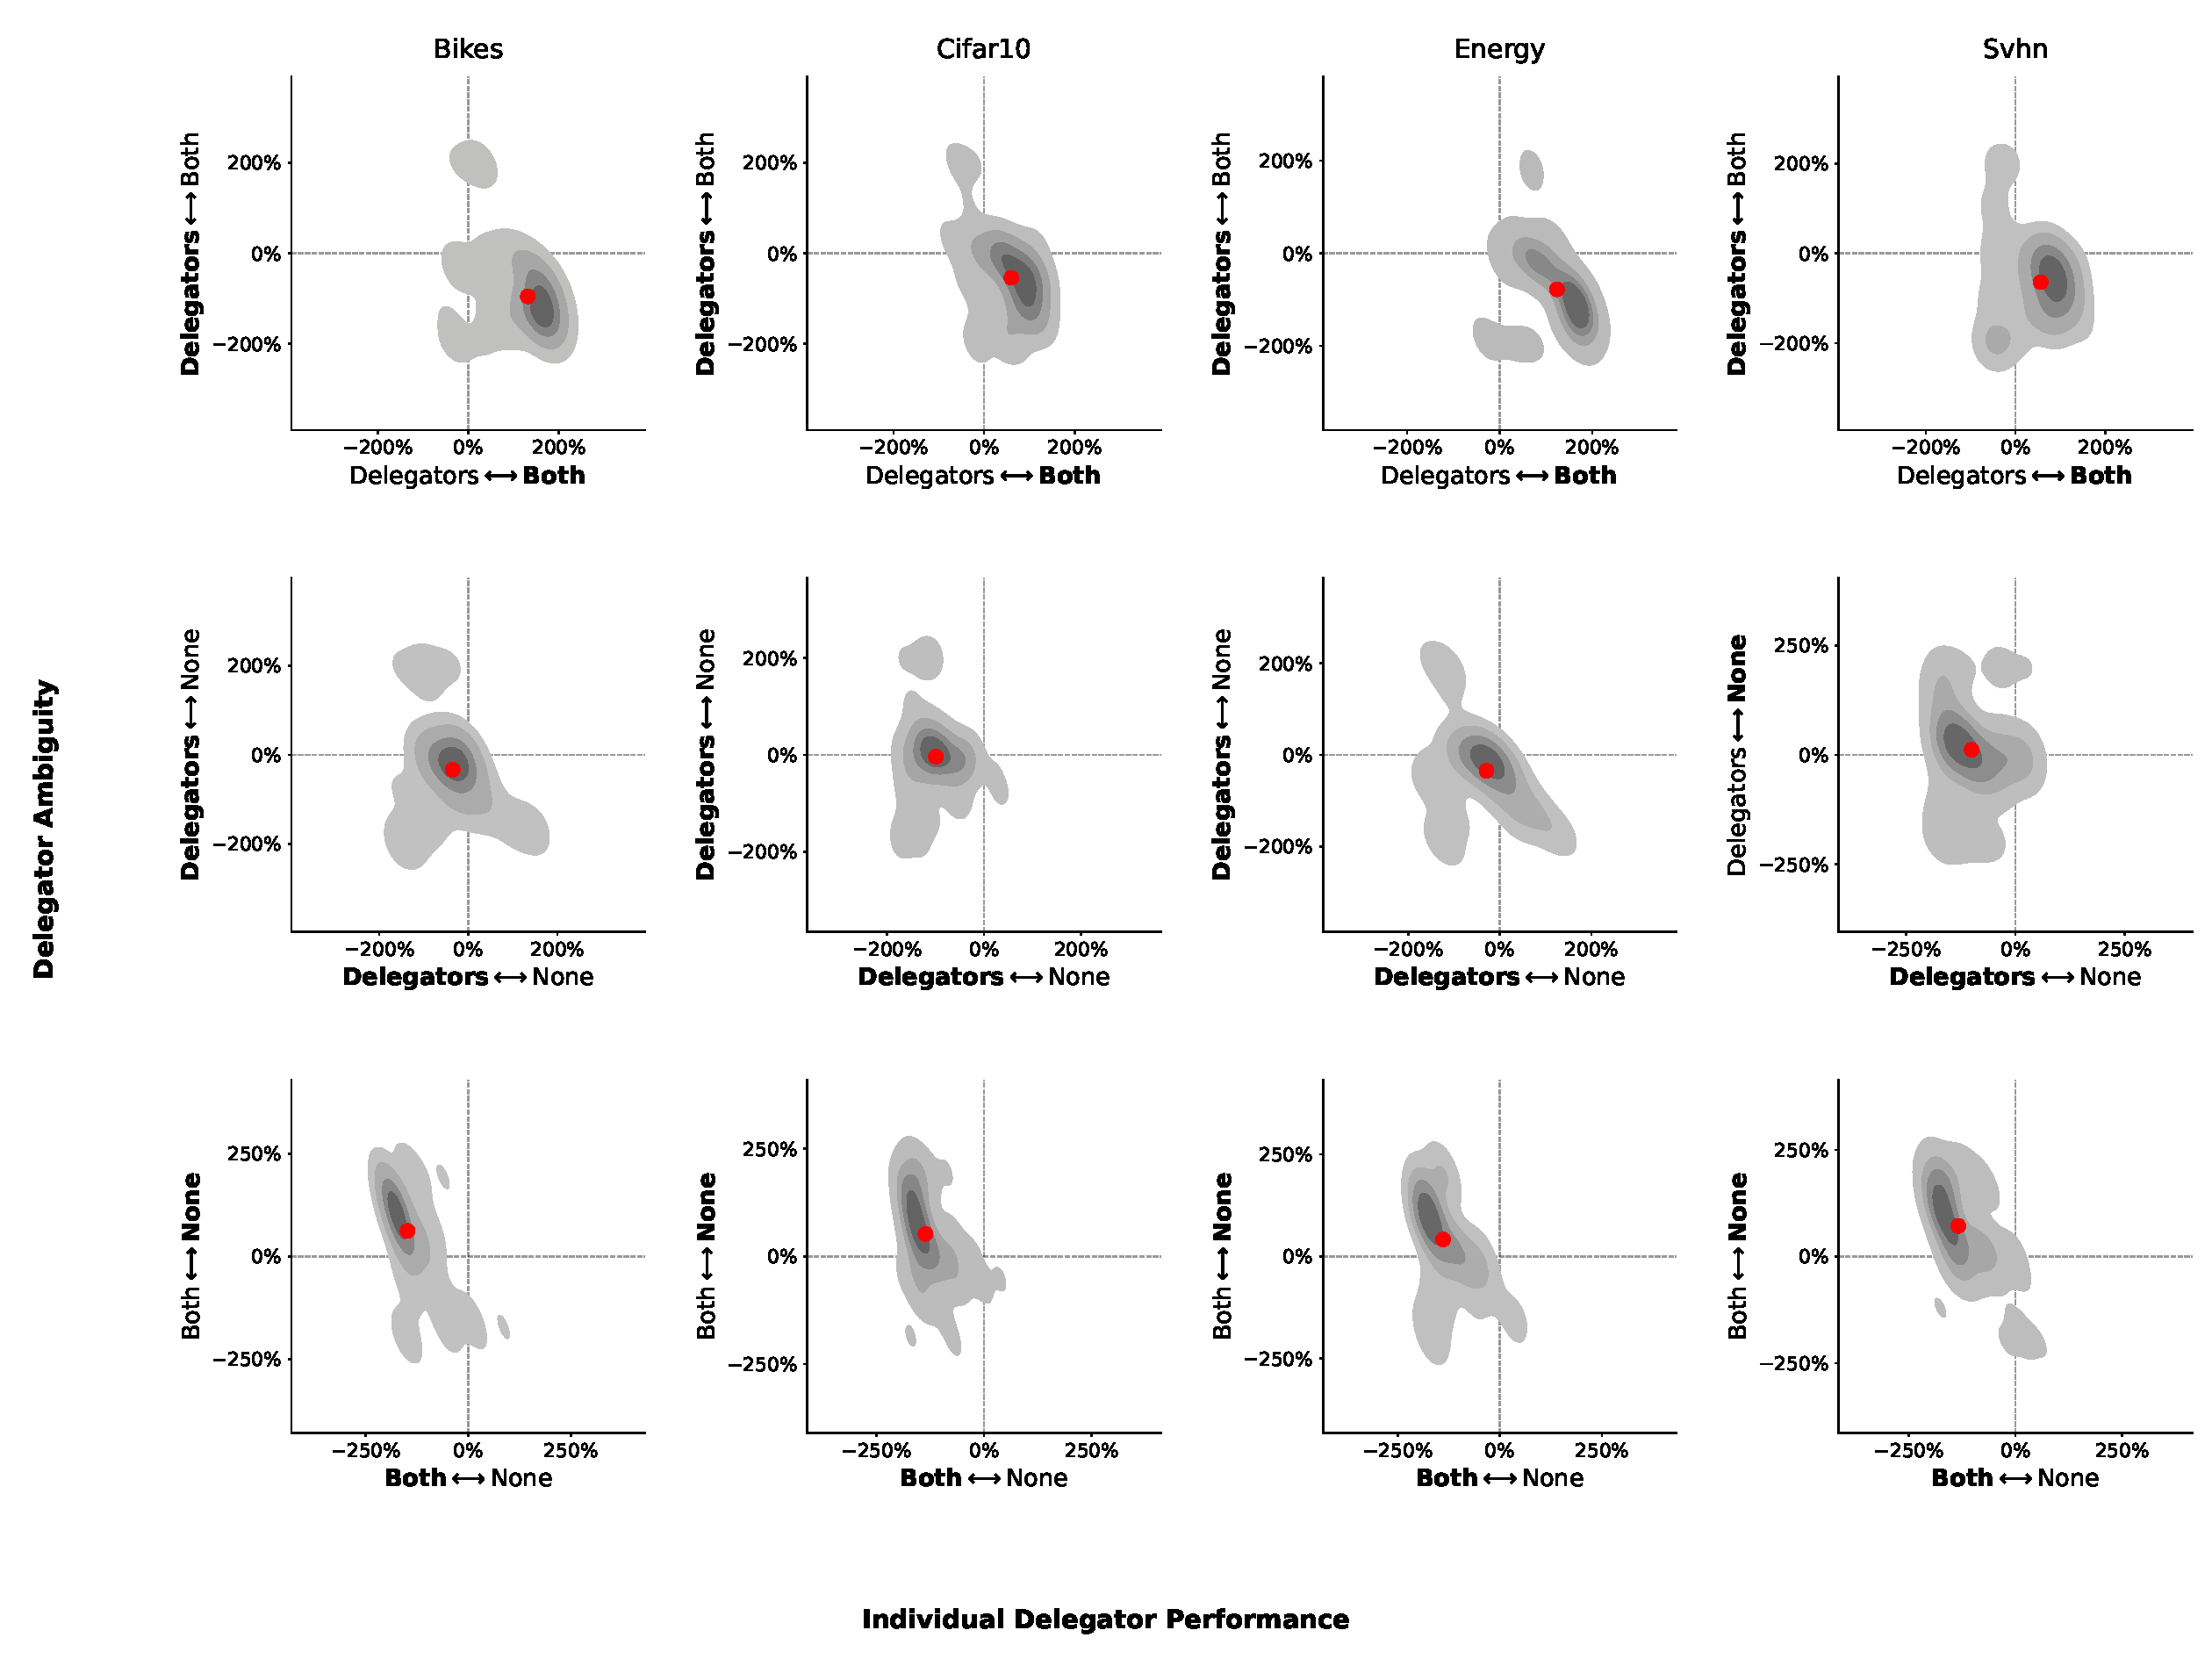
\includegraphics[width=0.99\linewidth]{figures/gradient_2ddist_delegators_ambiguity_performance.pdf}
    \caption{Ambiguity gradient flow: Distribution of the relative differences in individual delegator performance (x-axis; higher values indicate better performance) and delegator ambiguity (y-axis; higher values indicate greater ambiguity) across tasks and pairs of methods. The red dot denotes the distribution mean. For each task and method pair, the superior method is highlighted in bold.}
    \label{fig:placeholder}
\end{figure}

\paragraph{Delegators' regret analysis}

We found that in $85\%$ cases the restricted oracle was able to improve the validation loss.

\begin{figure}[h]
    \centering
    
\includegraphics[width=0.99\linewidth]{figures/gradient_box_regret_diff_bold_means_more_delegator_regret.pdf}
    \caption{Ambiguity gradient flow: Distribution of the relative differences in delegators' regret between pairs of ambiguity-gradient methods across tasks. Higher values indicate that a larger fraction of the remaining loss is attributable to the delegators. The black dot denotes the mean relative difference. For each task and method pair, the method with higher delegators' regret is highlighted in bold.}
    \label{fig:placeholder}
\end{figure}

\subsection{Delegator Ambiguity gradient flow} \label{sec:exp-delegator-gradient}

We next test whether delegators should be explicitly trained to increase their ambiguity. Joint ensemble training minimizes $\dperformance-\dambiguity$. Blocking the delegator-ambiguity gradient instead trains each delegator to produce an accurate ensemble prediction on its own, relying on different random initializations to induce diversity. We compare two settings, in which delegators receive gradients only from
\begin{equation}\label{eq:del-ambiguity-choices}
    \underbrace{\pperformance(\bar{\va})-\pambiguity(\bar{\va})}
        _{\text{Delegator ambiguity enabled}}
    \qquad\text{or}\qquad
    \underbrace{\dperformance}
        _{\text{Delegator ambiguity disabled}}.
\end{equation}
The first expression equals $\dperformance-\dambiguity$ and is only valid when predictor ambiguity gradient settings is not \texttt{None}. All other task-loss gradients to delegators are stopped; the load-balancing penalty remains active in both settings. The full training equations are annoyingly cumbersome, so we enumerate all combinations of predictor and delegator ambiguity gradient settings, including their stop-gradient operations, in Appendix~\ref{ap:gradient-routing}.

To isolate the effect of delegator ambiguity, we keep the predictor-ambiguity setting fixed at \texttt{Delegators} and use arithmetic delegator aggregation. We sample 100 configurations per task from the parameter sets in Table~\ref{tab:experiment-parameters}. For each configuration, we compare a matched pair with delegator ambiguity enabled or disabled, holding all other factors fixed. Each condition is evaluated over five independent random seeds. Across the four tasks, this yields 800 experimental conditions and 4,000 training runs.


\subsection{Analysis}

\bibliography{tmlr-template/tmlr}
\bibliographystyle{tmlr-template/tmlr}

\appendix

\section{Appendix}

\subsection{Training specifications} \label{ap:hyperparams}


\begin{table}[t]
\caption{Training and initialization hyperparameters used across experiments.}
\label{tab:training-hyperparameters}
\begin{center}
\begin{tabular}{ll}
\multicolumn{1}{c}{\bf HYPERPARAMETER}
&
\multicolumn{1}{c}{\bf VALUE}
\\ \hline \\
Kernel initialization          & LeCun normal \\
Bias initialization            & Zero \\
Hidden-layer activation        & ReLU \\
Optimizer                      & Adam \\
Learning rate                  & $10^{-3}$ \\
Weight-decay coefficient       & $10^{-4}$ \\
Tabular-task batch size        & $256$ \\
Image-task batch size          & $64$ \\
Tabular-task training epochs   & $2000$ \\
Image-task training epochs     & $50$ \\
\end{tabular}
\end{center}
\end{table}


\begin{table}[t]
\caption{Experimental values and their permitted set.}
\label{tab:experiment-parameters}
\begin{center}
\begin{tabular}{lll}
\multicolumn{1}{c}{\bf VARIABLE}
&
\multicolumn{1}{c}{\bf SET}
&
\multicolumn{1}{c}{\bf NOTES}
\\ \hline \\
Number of predictors ($M$) & \{$2, 4, 8, 16, 32$\} &  \\
Number of delegators ($L$) & \{$0, 1, 2, 4, 8, 16, 32$\} &  $L=0$: uniform weights; $L=1$: MoE. \\
Predictors' base width ($b_M$) & \{$4, 8, 16$\} & Predictor hidden layers are either $(2b,b)$ or $(3b,2b,b)$.  \\
Delegators' base width ($b_L$) & \{$4, 8, 16$\} & Delegator hidden layers are either $(2b,b)$ or $(3b,2b,b)$. \\
Delegators' aggregation method & \{mean, geometric mean\} & See Section \ref{sec:exp-agg} \\
Predictor ambiguity gradients & \{none, delegators, both\} & See Table~\ref{tab:gradient-flow}. \\
Delegator ambiguity gradient & \{disabled, enabled\} & Section~\ref{sec:exp-delegator-gradient}. \\
\end{tabular}
\end{center}
\end{table}



\subsection{Delegator performance--ambiguity decomposition under the sum rule}\label{ap:delegator-decomposition}

Fix a sample $(\vx,\vy)$ and $L\geq 1$ delegators. Under the sum rule, their weight proposals are averaged:
\begin{equation}
    \bar{\va}=\frac{1}{L}\sum_{l=1}^L\va_l,
    \qquad
    \hat{\vy}^{(l)}=F(\vx;\va_l),
    \qquad
    \hat{\vy}=F(\vx;\bar{\va}).
\end{equation}
We show that this rule makes the final prediction the appropriate aggregate of the delegator-induced predictions, and then derive $\ell(\hat{\vy},\vy)=\dperformance-\dambiguity$.

\paragraph{Regression.}
Predictor outputs are combined by a weighted arithmetic mean. Writing $a_{l,m}$ for the weight assigned to predictor $m$ by delegator $l$, we obtain
\begin{equation}
\begin{aligned}
    \hat{\vy}
    &=\sum_{m=1}^M\bar a_m\hat{\vy}_m
    =\frac{1}{L}\sum_{l=1}^L\sum_{m=1}^M a_{l,m}\hat{\vy}_m
    =\frac{1}{L}\sum_{l=1}^L\hat{\vy}^{(l)} \\
    \mathbf{0} &= \frac{1}{L}\sum_{l=1}^L\hat{\vy}^{(l)} - \hat{\vy} = \sum_{l=1}^L(\hat{\vy}^{(l)} - \hat{\vy})
\end{aligned}
\end{equation}
Expanding each individual squared error around $\hat{\vy}$ gives
\begin{equation}
\begin{aligned}
    \dperformance
    &=\frac{1}{Ld_y}\sum_{l=1}^L
      \left\|(\hat{\vy}^{(l)}-\hat{\vy})+(\hat{\vy}-\vy)\right\|_2^2\\
    &= \frac{1}{Ld_y}\sum_{l=1}^L \left\| \hat{\vy}^{(l)}-\hat{\vy} \right\|_2^2  + \frac{2}{Ld_y} (\hat{\vy}-\vy)^\top  \underbrace{\sum_{l=1}^L (\hat{\vy}^{(l)}-\hat{\vy})}_{\mathbf{0}}  + \frac{1}{Ld_y}\sum_{l=1}^L \left\| \hat{\vy}-\vy \right\|_2^2 \\
    &= \dambiguity + SE(\hat{\vy}, \vy)
\end{aligned}
\end{equation}
The cross term vanishes, yielding
\begin{equation}\label{eq:delegator-se-derivation}
    \mathrm{SE}(\hat{\vy},\vy)=\dperformance-\dambiguity.
\end{equation}

\paragraph{Classification.}
Predictor outputs are combined by a normalized weighted geometric mean. Assume positive predictor probabilities, so the logarithms below are defined. For class $c$, the prediction induced by delegator $l$ is
\begin{equation}
    \hat y_c^{(l)}
    =\frac{1}{Z_l}\prod_{m=1}^M\hat y_{m,c}^{a_{l,m}},
    \qquad
    Z_l=\sum_{c=1}^{d_y}\prod_{m=1}^M\hat y_{m,c}^{a_{l,m}}.
\end{equation}
Taking the geometric mean across delegators gives
\begin{equation}
    \prod_{l=1}^L\big(\hat y_c^{(l)}\big)^{1/L}
    =\left(\prod_{l=1}^L Z_l^{-1/L}\right)
      \prod_{m=1}^M\hat y_{m,c}^{\frac{1}{L}\sum_{l=1}^L a_{l,m}}
    =\left(\prod_{l=1}^L Z_l^{-1/L}\right)
      \prod_{m=1}^M\hat y_{m,c}^{\bar a_m}.
\end{equation}
The factor involving $Z_l$ is the same for every class and cancels when the probabilities are normalized. Hence the final prediction is the normalized geometric mean of the induced predictions:
\begin{equation}
    \hat y_c=\frac{1}{Z_{\mathrm{D}}}
      \prod_{l=1}^L\big(\hat y_c^{(l)}\big)^{1/L},
    \qquad
    Z_{\mathrm{D}}=\sum_{c=1}^{d_y}
      \prod_{l=1}^L\big(\hat y_c^{(l)}\big)^{1/L}.
\end{equation}
Taking logarithms yields
\begin{equation}
    \frac{1}{L}\sum_{l=1}^L\log\hat y_c^{(l)}
    =\log\hat y_c+\log Z_{\mathrm{D}}.
\end{equation}
Using $\sum_c y_c=1$, the mean individual delegator loss is therefore
\begin{equation}
\begin{aligned}
    \dperformance
    &=-\sum_{c=1}^{d_y}y_c
       \left(\frac{1}{L}\sum_{l=1}^L\log\hat y_c^{(l)}\right)\\
    &=\mathrm{CE}(\hat{\vy},\vy)-\log Z_{\mathrm{D}}.
\end{aligned}
\end{equation}
Similarly, using $\sum_c\hat y_c=1$, the mean delegator ambiguity is
\begin{equation}
\begin{aligned}
    \dambiguity
    &=\frac{1}{L}\sum_{l=1}^L
      \mathrm{KL}(\hat{\vy}\,\|\,\hat{\vy}^{(l)})\\
    &=\sum_{c=1}^{d_y}\hat y_c
      \left(\log\hat y_c-\frac{1}{L}\sum_{l=1}^L\log\hat y_c^{(l)}\right)
      =-\log Z_{\mathrm{D}}.
\end{aligned}
\end{equation}
Subtracting the two expressions gives
\begin{equation}\label{eq:delegator-ce-derivation}
    \mathrm{CE}(\hat{\vy},\vy)=\dperformance-\dambiguity.
\end{equation}
Equations~\ref{eq:delegator-se-derivation} and~\ref{eq:delegator-ce-derivation} establish Equation~\ref{eq:delegator-ambiguity}. Both rely on arithmetic aggregation of delegation weights; geometric weight aggregation does not generally produce the required mean of the induced predictions.

\subsection{Gradient routing}\label{ap:gradient-routing}

We enumerate all combinations of predictor ambiguity gradient (PAG) and delegator ambiguity gradient (DAG) settings. These abbreviations are used only in this appendix. We assume arithmetic delegation aggregation and $L\geq 1$, so the ensemble loss satisfies
\begin{equation}
    \ell
    = \pperformance(\bar{\va})-\pambiguity(\bar{\va})
    = \dperformance-\dambiguity,
    \qquad
    \dperformance
    = \frac{1}{L}\sum_{l=1}^L
      \left[\pperformance(\va_l)-\pambiguity(\va_l)\right].
\end{equation}

The operator $\sg_{\vTheta}$ preserves its argument's value but stops its gradient with respect to predictor parameters. Similarly, $\sg_{\vPhi}$ stops gradients with respect to delegator parameters, while $\sg$ stops all gradients. The expressions below define $\ell_{\mathrm{train}}$: each has the same numerical value as $\ell$, but supplies the gradients prescribed by its setting.

All settings also include the auxiliary losses, including the load-balancing penalty in Equation~\ref{eq:training-objective}. These are added unchanged and are not subject to the stop-gradient operations below.

\paragraph{PAG = Both, DAG = True}
Both predictors and delegators receive the full ensemble-loss gradient:
\begin{equation}
    \ell_{\mathrm{train}} = \ell.
\end{equation}

\paragraph{PAG = Delegators, DAG = True}
Predictor ambiguity updates only delegators:
\begin{equation}
    \ell_{\mathrm{train}}
    = \pperformance(\bar{\va})
      - \sg_{\vTheta}\left[\pambiguity(\bar{\va})\right].
\end{equation}

\paragraph{PAG = None, DAG = True}
Predictor ambiguity contributes no gradient:
\begin{equation}
    \ell_{\mathrm{train}}
    = \pperformance(\bar{\va})
      - \sg\left[\pambiguity(\bar{\va})\right].
\end{equation}

\paragraph{PAG = Both, DAG = False}
Predictors receive the full ensemble-loss gradient, while delegators learn only from their individual performance:
\begin{equation}
\begin{aligned}
    \ell_{\mathrm{train}}
    ={}& \sg_{\vPhi}\left[\ell\right]\\
       &+ \sg_{\vTheta}\left[
           \dperformance
           - \sg_{\vPhi}\left[\dambiguity\right]
           + \sg_{\vPhi}\left[\dambiguity-\dperformance\right]
         \right].
\end{aligned}
\end{equation}

\paragraph{PAG = Delegators, DAG = False}
Predictors learn only from their weighted individual performance. Delegators learn from their individual performance, which still accounts for predictor ambiguity:
\begin{equation}
\begin{aligned}
    \ell_{\mathrm{train}}
    ={}& \sg_{\vPhi}\left[
           \pperformance(\bar{\va})
           - \sg_{\vTheta}\left[\pambiguity(\bar{\va})\right]
         \right]\\
       &+ \sg_{\vTheta}\left[
           \dperformance
           - \sg_{\vPhi}\left[\dambiguity\right]
           + \sg_{\vPhi}\left[\dambiguity-\dperformance\right]
         \right].
\end{aligned}
\end{equation}

\paragraph{PAG = None, DAG = False}
Predictors learn only from their weighted individual performance. Delegators also ignore predictor ambiguity within each individual weight proposal:
\begin{equation}
\begin{aligned}
    \ell_{\mathrm{train}}
    ={}& \sg_{\vPhi}\left[
           \pperformance(\bar{\va})
           - \sg\left[\pambiguity(\bar{\va})\right]
         \right]\\
       &+ \sg_{\vTheta}\left[
           \frac{1}{L}\sum_{l=1}^L
           \left(
               \pperformance(\va_l)
               - \sg_{\vPhi}\left[\pambiguity(\va_l)\right]
           \right)
           - \sg_{\vPhi}\left[\dambiguity\right]
           + \sg_{\vPhi}\left[\dambiguity-\dperformance\right]
         \right].
\end{aligned}
\end{equation}

In the DAG = False settings, the second bracket has numerical value zero but supplies the required delegator gradients. The correction term $\sg_{\vPhi}[\dambiguity-\dperformance]$ therefore preserves the reported ensemble loss without changing either parameter group's updates.

\subsection{Restricted delegator oracle training procedure} \label{ap:restricted-oracle}

For candidate delegator parameters $\vPhi'$, let $\bar{\va}_{\vPhi'}(\vx)$ denote their aggregate weights. With predictors fixed, the oracle minimizes
\begin{equation}\label{eq:oracle-objective}
    \mathcal{L}_{\mathrm{oracle}}(\vPhi')
    = \frac{1}{|\sD_{\mathrm{fit}}|}
      \sum_{(\vx,\vy)\in\sD_{\mathrm{fit}}}
      \ell(F(\vx;\bar{\va}_{\vPhi'}(\vx)),\vy).
\end{equation}

For each trained seed, we freeze all predictor parameters and cache the validation predictions and each delegator's penultimate-layer features. Starting from the learned delegators, we fit only the kernels and biases of their final affine layers using full-batch L-BFGS with history size 10. The objective is Equation~\ref{eq:oracle-objective} with $\sD_{\mathrm{fit}}=\sD_{\mathrm{val}}$, without a routing tether, load balancing, weight decay, or ambiguity-gradient restrictions. We perform at most 100 updates and stop when the gradient norm is at most $10^{-6}$ or a nonfinite value is encountered. Each seed retains the weights with the lowest validation loss, including the unmodified initialization. The softmax routing makes this optimization generally nonconvex, so the resulting weights are a restricted reference rather than a certified optimum. Because validation labels participate in fitting and selection, this procedure quantifies recoverable loss on that dataset only.

\end{document}
